%\chapter{Intoduction to GameTheory}
%\label{cha:1}
\documentclass[10pt]{article}

\usepackage{graphicx}
\usepackage{amsmath}
\usepackage{listings}
\usepackage{color}
\usepackage{soul}
\usepackage{tikz}
\usepackage{parskip}
\usepackage{todonotes}
\usepackage{url}
\usepackage{natbib} 
\usepackage{pgf}
\usepackage{tikz}
\usetikzlibrary{arrows,automata}
%\usepackage[latin1]{inputenc}
\definecolor{dkgreen}{rgb}{0,0.6,0}
\definecolor{gray}{rgb}{0.5,0.5,0.5}
\definecolor{mauve}{rgb}{0.58,0,0.82}

\lstset{frame=tb,
  language=Java,
  aboveskip=3mm,
  belowskip=3mm,
  showstringspaces=false,
  columns=flexible,
  basicstyle={\small\ttfamily},
  numbers=none,
  numberstyle=\tiny\color{gray},
  keywordstyle=\color{blue},
  commentstyle=\color{green},
  stringstyle=\color{black},
  breaklines=true,
  breakatwhitespace=true
  tabsize=3
}

%\newcommand{\todo}[1]{{\huge \textcolor{green}{#1}}\\}
\newcommand{\com}[1]{\textcolor{red}{#1}\\}
\newcommand{\viscomment}[1]{\textcolor{red}{#1}}
\newcommand{\flip}[1] {\textcolor{black}{#1}}

% Tenslotte wordt hyperref gebruikt voor pdf bestanden.
% Dit mag verwijderd worden voor de af te drukken versie.
\usepackage[pdfusetitle,colorlinks,plainpages=false]{hyperref}

%%%%%%%
% Om wat tekst te genereren wordt hier het lipsum pakket gebruikt.
% Bij een echte masterproef heb je dit natuurlijk nooit nodig!
\IfFileExists{lipsum.sty}%
 {\usepackage{lipsum}\setlipsumdefault{11-13}}%
 {\newcommand{\lipsum}[1][11-13]{\par Hier komt wat tekst: lipsum ##1.\par}}

\begin{document}
\section{Write down the settings of the game}


%$N_{0}$ denotes the initially infected resources at the beginning of the virus propagation. 
%$P_{x}(R_{n},t|R_{0},r,t_{0})$ denotes the chance that resource $R_{n}$ is infected at time $t$ after dropping virus number x on to resource $R_{0}$ at $t_{0}$ with rate $r$. \\

%$S(R_{n},R_{0})$ denotes the shortest path from the infected resource $R_{0}$ to resource $R_{n}$. It gives back a value with the distance measured with how many resources are in between including the end resource. \\

%So the chance that a resource is infected after time t is the chance that the resource is infected by all the previous infections and that the defender has not flipped the resource.
source: \url{http://en.wikipedia.org/wiki/Adjacency_matrix} \\
We model the network through an undirected Graph $G = < V, E> $ where $|V|$ denotes the number of resources in the network and $|E|$ the number of connections. We can convert this to a adjacent matrix where we can represent which vertices of the graph are neighbours of other vertices. \\
For our graph we have an $|V| \times |V|$ matrix with on every entry $a_{ij}$ a 1 as value if there is a connection between node $V_{i}$ and $V_{j}$ and with zeros its diagonal. Because our graph is undirected we have a symmetric matrix. 

\textit{"If \textit{A} is the adjacency matrix of the directed or undirected graph \textit{G}, then the matrix $A^{n}$ (i.e., the matrix product of n copies of \textit{A}) has an interesting interpretation: the entry in row i and column j gives the number of (directed or undirected) walks of length n from vertex i to vertex j. If n is the smallest nonnegative integer, such that for all i ,j , the (i,j)-entry of $A^{n} > 0$, then n is the distance between vertex i and vertex j."} [Wikipedia]

%%% Local Variables: 
%%% mode: latex
%%% TeX-master: "thesis"
%%% End: 
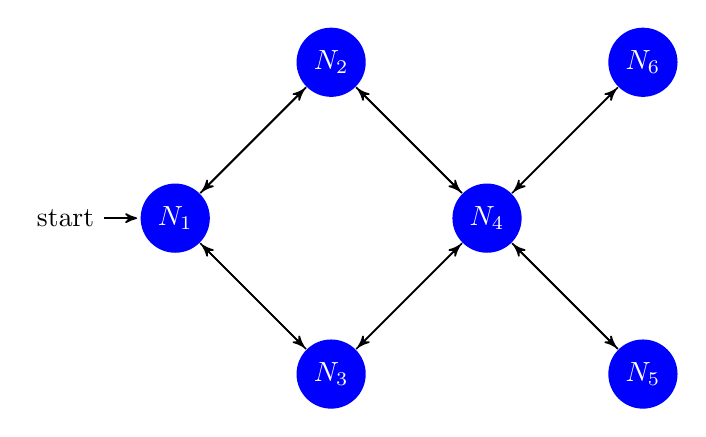
\begin{tikzpicture}[->,>=stealth',shorten >=1pt,auto,node distance=2.8cm,
                    semithick]
  \tikzstyle{every state}=[fill=blue,draw=none,text=white]

  \node[initial,state] (A)                    {$N_1$};
  \node[state]         (B) [above right of=A] {$N_2$};
  \node[state]         (D) [below right of=A] {$N_3$};
  \node[state]         (C) [below right of=B] {$N_4$};
  \node[state]         (E) [below right of=C] {$N_5$};
  \node[state]		   (F) [above right of=C] {$N_6$};

  \path (A) edge              node {} (B)
            edge              node {} (D)
        (B) edge              node {} (A)
        	edge			  node {} (C)
        (C) edge              node {} (B)
            edge 			  node {} (D)
            edge			  node {} (E)
            edge			  node {} (F)
        (D) edge 			  node {} (C)
            edge              node {} (A)
        (E) edge 			  node {} (C)
    	(F)	edge			  node {} (C);
\end{tikzpicture}
\\
%\[
%\begin{bmatrix}
%    x_{11}       & x_{12} & x_{13} & \dots & x_{1n} \\
%    x_{21}       & x_{22} & x_{23} & \dots & x_{2n} \\
%    \hdotsfor{5} \\
%    x_{d1}       & x_{d2} & x_{d3} & \dots & x_{dn}
%\end{bmatrix}
%=
%\begin{bmatrix}
%    x_{11} & x_{12} & x_{13} & \dots  & x_{1n} \\
%    x_{21} & x_{22} & x_{23} & \dots  & x_{2n} \\
%    \vdots & \vdots & \vdots & \ddots & \vdots \\
%    x_{d1} & x_{d2} & x_{d3} & \dots  & x_{dn}
%\end{bmatrix}
%\] 
The adjacent matrix becomes this matrix $[A]$: \\


$
\bordermatrix{
         & N_1		& N_2	& N_3	& N_4 	& N_5	&N_6     \cr
    N_1   & 0		& 1		& 1		& 0		& 0		& 0	     \cr
    N_2   & 1		& 0		& 0		& 1		& 0		& 0	     \cr
    N_3   & 1		& 0		& 0		& 1		& 0		& 0	     \cr
    N_4   & 0		& 1		& 1		& 0		& 1		& 1	     \cr
	N_5   & 0		& 0		& 0		& 1		& 0		& 0	     \cr
	N_6   & 0		& 0		& 0		& 1		& 0		& 0	     \cr
}$
\\

Matrix $A \times A = A^{2}$ becomes the matrix with the number of paths with 2 steps from $N_{i}$ to $N_{j}$: We denote this matrix as matrix \textit{[B]}\\


$
\bordermatrix{
         & N_1		& N_2	& N_3	& N_4 	& N_5	&N_6     \cr
    N_1   & 2		& 0		& 0		& 2		& 0		& 0	     \cr
    N_2   & 0		& 2		& 2		& 0		& 1		& 1	     \cr
    N_3   & 0		& 2		& 2		& 0		& 1		& 1	     \cr
    N_4   & 2		& 0		& 0		& 4		& 0		& 0	     \cr
	N_5   & 0		& 1		& 1		& 0		& 1		& 1	     \cr
	N_6   & 0		& 1		& 1		& 0		& 1		& 1	     \cr
}$
\\

Matrix $A^{2} \times A = A^{3}$ becomes the matrix with the number of paths with 3 steps from $N_{i}$ to $N_{j}$: We denote this matrix as matrix \textit{[C]}\\


$
\bordermatrix{
         & N_1		& N_2	& N_3	& N_4 	& N_5	&N_6     \cr
    N_1   & 0		& 4		& 4		& 0		& 2		& 2	     \cr
    N_2   & 4		& 0		& 0		& 6		& 0		& 0	     \cr
    N_3   & 4		& 0		& 0		& 6		& 0		& 0	     \cr
    N_4   & 0		& 6		& 6		& 0		& 4		& 4	     \cr
	N_5   & 2		& 0		& 0		& 4		& 0		& 0	     \cr
	N_6   & 2		& 0		& 0		& 4		& 0		& 0	     \cr
}$ 
\\

So for $A^{N}$ every $a_{ij}$ entry gives the number of paths with N steps from $N_{i}$ to $N_{j}$.\\

With this knowledge we can calculate in how many steps a node is infected. $A$ calculates which nodes are infected after 1 step, $A^{N}$ calculates which nodes are infected in N steps.. So if we want to know how many nodes are infected after 3 steps we have to add every matrix $(A + A^{2} + A^{3}) $ and see which entry is a non zero entry. 

What do we need for an algorithm
\begin{description}
\item Graph network $G = < V, E>$
\item Graph matrix $[A]$ which is $|V| \times |V| $
\item Attack vector $[X]$ which is $1 \times |V|$
\item cummulative matrix $[M]$ which is $|V| \times |V|$
\item state matrix $[T]$  which is $|V| \times |V|$
\item Reset vector $[R]$
\item duration \textit{d}
\item time \textit{n}
\item rate $\delta _{0}$ of defender and $\delta _{1}$ of attacker
\end{description}



Initialisation algorithm:


\begin{verbatim}
initialisatie
	d=0
	A=basismatrix
	M=A^{0}
	n=0
	\delta_{0}
	\delta_{1}
	X
	R
	controller = defender
	
	

	Algorithm
	n:= n + 1;
	Check who is in control? ( through modulo )
	if ( defender & controller=defender)
				d:= d + 1;
	
	if ( defender & controller=attacker )
				G = X \times R  (flippen ten voordele van defender)
				d = 0
				controller = defender
				
	if ( attacker & controller=defender )
				controller=attacker
				..
				
	if ( attacker & contoller=attacker )
				d:= d + 1
				M = M x A
				T = T + M
				G = X x T
				
		
\end{verbatim}

\end{document}